\documentclass{article}
\usepackage[preprint]{ge2340_project}
\usepackage[utf8]{inputenc}
\usepackage[T1]{fontenc}
\usepackage{url}
\usepackage{booktabs}
\usepackage{longtable}
\usepackage{amsmath,amssymb}
\usepackage{graphicx}
\usepackage{microtype}
\usepackage{xcolor}
\usepackage{float}
\usepackage{hyperref}
\setcitestyle{numbers,square}
\hypersetup{colorlinks=true,linkcolor=blue,citecolor=blue,urlcolor=blue,
  pdftitle={Phase 2: Course Registration Helper for Balanced Workloads},pdfauthor={}}
\urlstyle{same}
\title{Phase 2: AI Project Report\\
\large Course Registration Helper for Balanced Workloads}
\author{}

\begin{document}
\maketitle

\section{Introduction \& Problem Recap}
Study-path planning is an important progress in university life.However, for some students in city university unfamiliar with GE or elective courses ,such as its background requirements, workload. While seats are limited, students often have to make a rush decision for which course to register. And there is a more often appears that: originally there is no seats at the before the semester start. After the first week, some other students in certain dropped the course, which free up the seats. However, the students who failed to register any GE courses ,rush to register the courses with new free space. But they may get into a course which difficult to them at week 2, where the add-drop period has been ended, make the decision become no no-regret.
Our helper uses an LLM and course scoring to suggest suitable, workload-aware schedules from students' interests, year and required courses. The prototype covers selected courses in one semester; it supports course selection rather than automatic registration or guaranteed seats.

Our design combines a fine-tuned language model with mathematical optimisation. The model interprets course information and proposes structured recommendations; source checks and an optimiser turn them into a constrained plan. This lets us personalise recommendations while respecting programme eligibility and academic dependencies.



\section{Data Collection \& Methodology}
\textbf{A programme-specific knowledge base.} Due to the time limitation and workload, we trained the data of BSc in Computing Mathematics (CM) and BSc in Computer science (CS) to the model.We assembled the student handbook, CM degree path and course list, CS major requirements and suggested plan, GE information, and saved Semester A/B timetable pages\citep{cityu-programmes}. We preserve source cohorts and academic years: the CM path concerns the 2025 intake, its designated course list is historical, and CS requirements and its suggested plan cover different academic-year contexts. These distinctions remain visible when rules need confirmation.

\begin{table}[H]
\centering\small
\caption{Coverage of our programme and timetable collection.}
\begin{tabular}{p{3.85in}r}
\toprule
Knowledge-base component & Coverage\\
\midrule
Distinct timetable files after duplicate removal & 93\\
Course--term--programme records & 86\\
Sections matching the encoded major restrictions & 128\\
CM / CS document-listed course codes & 85 / 73\\
GE codes in the original import & 64\\
Files excluded because meeting times were unrecognised & 7\\
\bottomrule
\end{tabular}
\label{tab:data}
\end{table}

\textbf{Turning documents into usable rules.} We extracted meeting days/times, prerequisites, exclusions and restrictions, removed duplicates and retained sources. ``ONLY FOR CM'' is an explicit major restriction. Candidates must appear in the student's designated programme document or the verified GE collection, then satisfy further eligibility checks. Entries with missing times are excluded from verified timetable planning. 

\newpage
\textbf{Training and evaluation design.} Our initial programme dataset contains 485 training, 24 validation and 30 test examples combining curriculum/timetable extraction with synthetic stream-policy answers. Its before/after comparison uses 15 preselected queries across membership, sections, course rules, source extraction and stream reasoning. The CM finance-background update uses 244 training and 32 validation examples, plus 20 held-out profile/candidate combinations. Both comparisons use the same base-loading protocol for each pair. Shared source facts and synthetic policies mean these are familiar-evidence tests, rather than unseen-cohort evaluations.

We complement this comparison with controlled penalty experiments, dependency interventions with fictional student profiles. Fictional transcripts let us vary academic histories without using real student records. Workload and preparation scores are transparent, editable estimates,with human feedback on the parameters. 

After the round of the training, we will give human feedback on the generated example to fine-tune the model further more.
\textbf{Prompts used in training.} Our saved training rows contain three message roles: a system instruction defining the task and output rules, a user message supplying the programme, passed courses, source facts and requested task, and an assistant message containing the target JSON. Instructions include ``Return JSON only,'' preserve source times, distinguish documents from instructions, count distinct stream slots, and never infer passes from year of study. The CM background prompt also states the EF/CS planning waiver and the treatment of failed/in-progress finance records. We train on assistant-answer tokens using supervised cross-entropy; this is more than providing a prompt at inference time.

\section{Implementation Details}
\textbf{From student profile to explained recommendation.} Our pipeline combines course evidence, the student's passed courses and their preferences. The language model returns structured proposals, which we check against exact local rules. The planner then evaluates eligible options and explains the selected route, reward contributions and unresolved requirements (Figure~\ref{fig:workflow}). A rejected model answer can be replaced by source lookup or exact policy calculation, with that intervention recorded separately.

\begin{figure}[H]
\centering
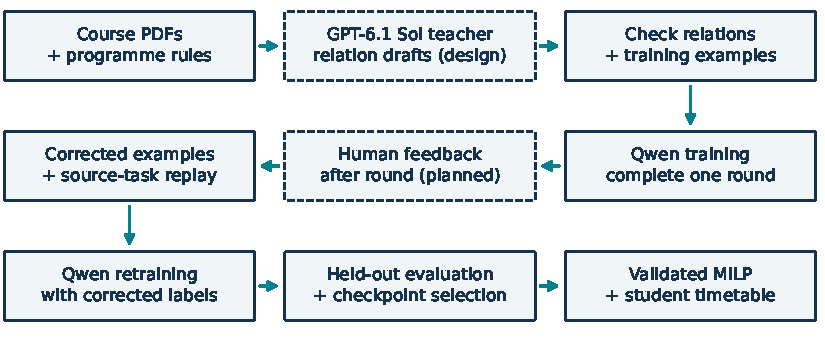
\includegraphics[width=\linewidth]{figures/workflow_training03.pdf}
\caption{Expanded training workflow: GPT relation teaching and post-round human feedback feed Qwen retraining, followed by validation and timetable optimisation. Dashed boxes denote designed feedback stages whose separate execution is not established by the saved training logs.}
\label{fig:workflow}
\end{figure}

\begin{samepage}
\textbf{GPT-6.1 Sol teaching course relations.} In the teacher-guided design, GPT-6.1 Sol reads the supplied course information and proposes relation examples: shared mathematical preparation, finance/AI interest links, workload implications and prerequisite bridges. We separate official requirements from inferred content links, review the proposed labels, and teach Qwen with the accepted source-conditioned input/output examples. A relation is an editable preparation hypothesis, not automatic registration permission. This is teacher-output distillation; we do not claim that Qwen also trains GPT.

\end{samepage}

\textbf{Human feedback after a full training round.} After one complete model-to-model teaching round and evaluation, a reviewer checks generated relations, rewards and schedules. Incorrect examples receive corrected targets and explanations; correct source examples are replayed to reduce forgetting. We then retrain Qwen and retain a checkpoint only if held-out checks support it. The repository demonstrates supervised training and corrective replay, but does not contain a separately logged GPT relation-teaching trial or a formal human-annotation evaluation; these two workflow stages remain a protocol for the next review cycle.

\textbf{Efficient model adaptation.} We fine-tuned Qwen3-8B\citep{qwen} using rank-8 QLoRA\citep{qlora}, with a frozen four-bit base and BF16 computation. This adapts approximately 21.8 million parameters on a single RTX 5090. The finance-background fine-tune completed two epochs in approximately 5.5 minutes, with 7.37 GiB peak allocated GPU memory. Validation loss decreased from 0.13366 to 0.00135. We retained the first epoch because its validation result was better than the second.

We use supervised cross-entropy to teach structured responses. The planner's academic-profit objective is a separate optimisation function: training teaches the model to express the relevant information, while the optimiser decides which feasible course combination best fits the student's preferences. This separation makes preference changes immediate without requiring retraining.

\textbf{Input control.} Our local interface accepts a transcript profile, a desired stream, a stream-priority weight and three penalty weights. It provides course lookup, stream proposals, dependency paths and semester planning. The optimiser uses SciPy's mixed-integer linear programming interface\citep{scipy}. We retain experiment inputs, outputs and policy decisions so recommendations can be traced back to the evidence\citep{runs}.

\newpage
\textbf{Reward and penalty function } 
Consider the penalty function 
\[
  \min_{\mathbf{x}}\;\sum_i x_i
  \bigl(\lambda_b b_i+\lambda_d d_i+\lambda_w w_i\bigr)
 \]
With binary course-selection variables $x_i$,and $b_i,d_i,w_i$ are mismatch, difficulty and workload scores, and the non-negative $\lambda$ values express student priorities.We try to minimize the penalty due to above factors.\\
Now, assume the reward for picking certain course be $R_i$ ,our objective function become 
\[\max_{\mathbf{x}}\;\sum_i x_iR_i \text{ subject to }\min_{\mathbf{x}}\;\sum_i x_i
  \bigl(\lambda_b b_i+\lambda_d d_i+\lambda_w w_i\bigr)\]
which is equivant to
\[\max_{\mathbf{x}}\;\sum_i x_iR_i  -x_i
  \bigl(\lambda_b b_i+\lambda_d d_i+\lambda_w w_i\bigr)\]
and the whole schedule can be written in a Markov decision process.\\
\textbf{Final formula for the Markov decision process}
Let $s$ describe the student's completed courses, covered GE areas, year, credit progress and selected stream. For a feasible course set $X$, we maximise
\begin{align}
U(X,s)={}&\sum_{c\in X}\bigl[g_c(s)+p_c(s)+h_c(s)+q_c(s)\nonumber\\
&\quad-\lambda_b b_c(s)-\lambda_d d_c(s)-\lambda_w w_c(s)\bigr]
+R_{\mathrm{stream}}(X,s)-O(X,s). \label{eq:utility}
\end{align}
The positive terms reward base course value $g$, preparation $p$, graduation priorities $h$, prerequisite bridges $q$ and progress towards one selected stream $R_{\mathrm{stream}}$. The three non-negative weights $\lambda_b,\lambda_d,\lambda_w$ control penalties for background mismatch, difficulty and workload. Profit is expressed in academic-utility points. Minimising the planner's loss is equivalent to minimising $-U$.
\\\textbf{overload penalty} To restrict the maximum credit that taken in a semester, we introduce overload penalty function
\begin{equation}
O(X,s)=\begin{cases}
0.25[\max(0,C(X)-15)]^2,&\text{Years 1--3},\\
0.25[\max(0,C(X)-12)]^2,&\text{Year 4}.
\end{cases}
\end{equation}
where $C(X)$ is semester credits. In Years 1--3 the penalty is zero through 15 credits, then 0.25 at 16 credits and 2.25 at 18 credits. In Year 4 it is zero through 12 credits, then 2.25 at 15 and 9 at 18 credits. We use the same 0.25 coefficient for the newly added earlier-year term. Inspection found that the previous default disabled overload penalties in Years 1--3; we corrected both the semester optimiser and the four-year simulation. This is a planner-policy correction, not a claim that the saved neural weights were retrained on this new threshold. The 18-credit hard limit remains separate.

\textbf{Personalisation across a degree} During the first round of training, we used GPT-6.1 Sol to deduce the relation between course and course. For example, a student who studied GE2340 can reward higher reward on furture AI -related course. Meanwhile, for GE course, if a student has already
covered its GE area, another distributional GE in that area receives only 0.3 base profit, encouraging breadth. A selected stream earns 2 points per new distinct requirement slot and a one-time 6-point completion reward. 

We account for both immediate progress and the next step in a course chain. For example, a prerequisite bridge can receive extra reward because it opens access to a preferred stream. Stream slots and completion rewards are counted once, including when several alternatives are selected together. In four-year simulations, the student's state is updated after each semester, allowing later decisions to reflect earlier choices.


\textbf{Background-focused CM planning.} For CM students, our planner allows an assumed prerequisite waiver for the listed EF and CS courses. Missing those formal passes adds no extra penalty. We instead assess finance preparation: background mismatch is 0.45 without evidence, 0.15 for introductory study and 0.05 for advanced passed study. Passed finance GEs or an explicit study declaration can supply introductory evidence; failed/in-progress courses do not. This is an advisory assumption, not verified university waiver approval.

\textbf{Academic requirements remain binding.} Programme membership, exclusions, required courses, credit bounds, section restrictions and timetable conflicts still apply. Mathematics and non-CM prerequisites remain enforced. Defaults require 5--6 courses in Years 1--3, with at most 18 credits; the Year 4 minimum is waived. Distributional GE is capped at one per semester, excluding compulsory language/development courses. Our CM degree simulation targets at least 122 credits, four distributional GEs spanning all three areas and at least 20 elective mathematics credits outside core/capstone study. The source's 122-credit threshold also meets the requested 121-credit minimum.

Unknown component linkage or teaching weeks is flagged. Hypothetical timetable examples explicitly state their assumptions, and dependency layers describe academic order rather than guaranteed future semester offerings. These boundaries help students distinguish a useful planning route from confirmed registration availability.

\newpage
\section{Results \& Evaluation}

\textbf{Year 2 profiles and Year 3 Semester A decisions.} We ran a fresh blind comparison on six fictional Year 2 students, using their projected end-of-Year-2 passing transcripts to plan Year 3 Semester A. Neither model saw the other's output or the reference solution. The saved Semester A 2026 course options are used as a planning proxy; actual Semester A 2027 offerings are unverified. Table~\ref{tab:year3-input06} gives every completed-course profile and the resulting next-semester selection. Table~\ref{tab:future-effects06} then compares how matched profile differences change the later academic path. No meeting times are shown.

{\small
\setlength{\tabcolsep}{4pt}
\renewcommand{\arraystretch}{1.12}
\begin{longtable}{p{2.45in}p{1.35in}p{1.35in}}
\caption{Completed Year 2 profiles and Year 3 Semester A course selections.}\label{tab:year3-input06}\\
\toprule
Year 2 student: completed courses and preference & Fine-tuned Qwen: Year 3 A & GPT-6.1 Sol: Year 3 A\\
\midrule
\endfirsthead
\multicolumn{3}{l}{\textit{Continued}}\\
\toprule
Year 2 student: completed courses and preference & Fine-tuned Qwen: Year 3 A & GPT-6.1 Sol: Year 3 A\\
\midrule
\endhead
\midrule
\multicolumn{3}{r}{\textit{Continued on next page}}\\
\endfoot
\bottomrule
\endlastfoot
{\raggedright \textbf{CM1; CM.} Passed: CS1302, CS2360, CS2468, GE1401, GE1501, GE2260, GE2401, MA1300, MA1301, MA2503, MA2507, MA2508, MA2509, MA2510, MA3511, MA3526. \textit{Preference:} Financial Mathematics.\par} & {\raggedright MA3521, MA3525, EF3320$^{\dagger}$\par} & {\raggedright MA3512, MA3518, MA3521, MA3525, MA4545\par}\\
\addlinespace[3pt]
{\raggedright \textbf{CM2; CM.} Passed: CS1302, CS2360, CS2468, GE1401, GE1501, GE2260, GE2401, MA1300, MA1301, MA2503, MA2507, MA2508, MA2509, MA2510, MA3511. \textit{Preference:} Financial Mathematics.\par} & {\raggedright MA3521, MA4545, MA3525\par} & {\raggedright MA3512, MA3518, MA3521, MA3525, MA4545\par}\\
\addlinespace[3pt]
{\raggedright \textbf{CM3; CM.} Passed: CS1302, CS2360, CS2468, GE1401, GE1501, GE2260, GE2401, MA1300, MA1301, MA2503, MA2507, MA2508, MA2509, MA2510, MA3511, MA3526. \textit{Preference:} Enriched Mathematics.\par} & {\raggedright MA3512, MA3518, MA4542, MA4545\par} & {\raggedright MA3512, MA3518, MA3525, MA4542, MA4545\par}\\
\addlinespace[3pt]
{\raggedright \textbf{CS1; CS.} Passed: CS1302A, CS2115, CS2310, CS2312, CS2402, CS3103, CS3201, CS3334, CS3342, GE1401, GE1501, GE1601, GE2340, MA1503, MA1508, MA2185. \textit{Preference:} Artificial Intelligence.\par} & {\raggedright CS3383, CS3402, CS3356\par} & {\raggedright No feasible five-course plan in supplied pool\par}\\
\addlinespace[3pt]
{\raggedright \textbf{CS2; CS.} Passed: CS1302A, CS2115, CS2310, CS2312, CS2402, CS3103, CS3201, CS3334, GE1401, GE1501, GE1601, GE2340, MA1503, MA1508, MA2185. \textit{Preference:} Artificial Intelligence.\par} & {\raggedright CS3402, CS3483\par} & {\raggedright No feasible five-course plan in supplied pool\par}\\
\addlinespace[3pt]
{\raggedright \textbf{CS3; CS.} Passed: CS1302A, CS2115, CS2310, CS2312, CS2402, CS3103, CS3201, CS3334, CS3342, GE1401, GE1501, GE1601, GE2340, MA1503, MA1508, MA2185. \textit{Preference:} Data Science.\par} & {\raggedright CS2613, CS3402, CS3483\par} & {\raggedright No feasible five-course plan in supplied pool\par}\\
\addlinespace[3pt]
\end{longtable}
}

\noindent\footnotesize All six inputs are Year 2 profiles; all selections target Year 3 Semester A. $\dagger$ Qwen returned an option ID outside the supplied candidate set. Outputs are preserved as generated, including incomplete or unsupported selections; no automatic correction is substituted.\normalsize

\newpage
{\small
\setlength{\tabcolsep}{4pt}
\renewcommand{\arraystretch}{1.12}
\begin{longtable}{p{1.05in}p{2.05in}p{2.05in}}
\caption{How completed study and stated preferences affect the later path: matched-profile observations.}\label{tab:future-effects06}\\
\toprule
Profile factor & Fine-tuned Qwen: observed later path & GPT-6.1 Sol: observed later path\\
\midrule
\endfirsthead
\multicolumn{3}{l}{\textit{Continued}}\\
\toprule
Profile factor & Fine-tuned Qwen: observed later path & GPT-6.1 Sol: observed later path\\
\midrule
\endhead
\midrule
\multicolumn{3}{r}{\textit{Continued on next page}}\\
\endfoot
\bottomrule
\endlastfoot
{\raggedright Analysis pass: CM1 versus CM2\par} & {\raggedright CM1 proposes MA4529 and later options, but incorrectly includes MA4542/MA4545 among finance options. CM2 shifts toward EF3320/EF4821 and does not identify recovery of missing MA3526.\par} & {\raggedright The immediate Year 3 A selection is unchanged. Both paths continue toward MA4529 and finance options, but CM2 explicitly requires MA3526 before analysis-dependent upper-level study.\par}\\
\addlinespace[5pt]
{\raggedright Explicit CM stream: CM1 versus CM3\par} & {\raggedright With the same completed courses and finance GE, the Enriched preference changes the selection toward MA4542/MA4545 and the later proposal to MA3523 plus MA4546/MA4551.\par} & {\raggedright The Enriched preference replaces MA3521 with MA4542 in Year 3 A. The later route changes from finance courses to MA3523 plus one of MA4528, MA4546 or MA4551, conditional on passing the selected courses.\par}\\
\addlinespace[5pt]
{\raggedright CS3342 pass: CS1 versus CS2\par} & {\raggedright CS1 proposes CS3383 and later AI core study. When CS3342 is missing, CS2 still proposes later CS4486/CS4487 and CS4386/CS4490 without a CS3342-recovery step.\par} & {\raggedright CS1 can access CS3383, but the current proxy pool has a clash that prevents a five-course plan. CS2 has only three distinct candidates and needs CS3342 recovery before CS3383, plus a revised candidate pool.\par}\\
\addlinespace[5pt]
{\raggedright Explicit CS stream: CS1 versus CS3\par} & {\raggedright With the same completed courses and AI GE, the Data Science preference changes the later proposal from CS4486/CS4487 toward CS3481, CS4480 and CS4487.\par} & {\raggedright The later goal changes from AI core CS4486/CS4487 to the Data Science chain CS3481, CS4480 and CS4487. Neither profile has a complete feasible plan in the supplied Semester A pool.\par}\\
\addlinespace[5pt]
\end{longtable}
}

The second table summarises the models' returned explanations and the observed course-set changes; it does not certify stream completion or future availability. In particular, changing a profile can alter the later prerequisite-recovery advice without changing the immediate semester selection, as CM1 versus CM2 demonstrates.

\textbf{Three penalties give students meaningful control.} We tested six penalty settings on matched CM and CS fixtures. Four required three-credit courses, three alternative electives, scores and synthetic times remain fixed; only the weights change. Each resulting optimum was independently checked by enumerating the three alternatives.

\begin{table}[H]
\centering\small
\caption{Changing the three penalties changes the preferred elective. Each setting was tested separately for CM and CS with matched synthetic scores.}
\begin{tabular}{cccp{1.05in}p{1.05in}r}
\toprule
$\lambda_b$ & $\lambda_d$ & $\lambda_w$ & CM elective & CS elective & Net utility\\
\midrule
1 & 1 & 1 & MA3521 & CS4486 & 17.25\\
20 & 1 & 1 & MA3521 & CS4486 & 1.10\\
1 & 20 & 1 & MA3523 & CS3483 & $-5.90$\\
1 & 1 & 20 & MA3525 & CS3402 & $-5.75$\\
0 & 12 & 1 & MA3523 & CS3483 & 2.85\\
12 & 12 & 1 & MA3521 & CS4486 & $-8.05$\\
\bottomrule
\end{tabular}
\label{tab:lambda}
\end{table}

A stronger difficulty penalty selects MA3523/CS3483, while a stronger workload penalty selects MA3525/CS3402. A larger background penalty can change utility without changing the chosen course. All 12 constructed optima pass verification. Negative utility reflects binding study requirements under a demanding preference setting; values across different weight settings are not directly comparable measures of educational quality.

\textbf{Dependency experiment: how earlier study changes a reward.} We designed 12 paired interventions to isolate individual dependencies. Year, base profit, score vector and penalty weights remain fixed; credit-progress and overload effects are excluded. Table~\ref{tab:dependency} summarises the observed changes. All 12 match their predeclared policy effects.

\begin{table}[H]
\centering\small
\caption{Dependency effects with other utility components held fixed. Deltas are configured utility points. A prerequisite can unlock a course without increasing its numeric reward.}
\begin{tabular}{p{2.2in}p{0.65in}p{2.15in}}
\toprule
Changed history or preference & Target & Observed effect\\
\midrule
Pass MA2508 & MA3515 & Preparation reward $+0.20$\\
Pass MA2509 & GE2134 & Preparation reward $+0.15$\\
Replace Area-2 GE with Area-1 GE & GE1113 & Same-area base reward $-2.70$\\
Pass GE2260; finance selected & MA3521 & Stream reward $+4.00$\\
Pass GE2260; explicit Enriched choice & MA3521 & No reward change\\
Pass CS3481 & CS4487 & Prerequisite unlocked; reward unchanged\\
Pass CS4480; CS3481 already passed & CS4487 & Final-slot completion reward $+6.00$\\
Pass unrelated GE1305 & MA3521 & No reward change\\
Duplicate a passed MA2509 ID & GE2134 & No repeated preparation reward\\
Pass GE2260; finance bridge pending & MA2510 & Bridge reward $+2.00$\\
Pass GE2260; finance weight already 3 & MA3521 & No second preference multiplier\\
Pass MA2503; conceptual finance link & EF3320 & No preparation bonus from this link\\
\bottomrule
\end{tabular}
\label{tab:dependency}
\end{table}

\newpage
\textbf{Recognising a complete course chain.} We also tested an interaction in the Software Engineering and Project Management stream. The target CS4348 earns 2 stream points with neither CS3346 nor CS3356 passed, or with either one passed alone. With both passed, CS4348 becomes the final requirement and earns 8 points. The interaction $8-2-2+2=6$ correctly isolates the completion reward. All four model queries reproduce the expected policy answers (Figure~\ref{fig:interaction}). These are computational rule tests; source-date and offering restrictions still apply.

\begin{figure}[H]
\centering
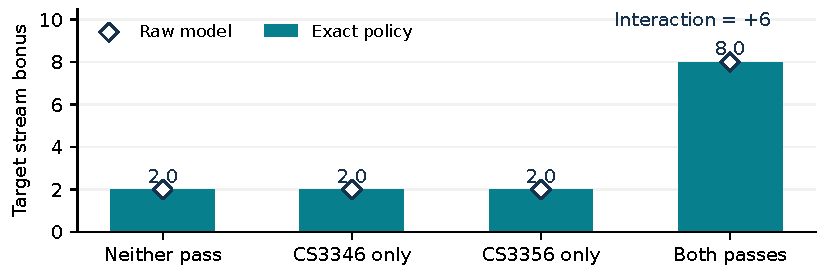
\includegraphics[width=\linewidth]{figures/stream_interaction.pdf}
\caption{Our model reproduces the stream-completion threshold in all four controlled cases. The additional six points reward finishing the chain.}
\label{fig:interaction}
\end{figure}

Grade controls reinforce this behaviour: a passed MA2509 receives its preparation benefit, while failed, in-progress and withdrawn records do not. Prerequisite-OR checks also recognise that either qualifying alternative is sufficient. These results validate our configured mechanisms; measured workload or learning benefits require a student study. An end-to-end schedule intervention remains future work, because a reward change does not necessarily change the best feasible timetable.

\textbf{Personalised paths across 20 student profiles.} We generated ten CM and ten CS fictional profiles with taught core completed, random GE histories and balanced desired-stream choices. With the CM waiver rule, our path checker produces 11 academic dependency paths, five advisory paths assuming the waiver and four provisional paths requiring further rule confirmation. Representative outputs appear in Table~\ref{tab:examples}. Capstones, internships and future offerings are not assumed satisfied.

\begin{table}[H]
\centering\small
\caption{Examples of the paths and obstacles our helper explains. Arrows indicate academic dependency order.}
\begin{tabular}{p{1.4in}p{2.2in}p{1.4in}}
\toprule
Student preference & Recommended route or identified obstacle & Planning result\\
\midrule
CM: Enriched Mathematics & MA3523, MA4542, MA4545 and MA4546 & Academic path\\
CS: Artificial Intelligence & CS3383 + CS4486 $\rightarrow$ CS4487 & Academic path\\
CS: Data Science & CS3402 + CS3481 $\rightarrow$ CS4480 + CS4487 & Bridge courses needed\\
CM: Financial Mathematics & {\raggedright MA3521, MA4529 + two of MA4537, EF3320 or EF4821\par} & Waiver assumed\\
\bottomrule
\end{tabular}
\label{tab:examples}
\end{table}

Before the finance-focused update, the model passed exact stream-policy validation in 10/20 of these profiles: 0/10 CM and 10/10 CS. Rejected answers used exact policy outputs. This historical result identifies the reasoning gap that motivated further training; the updated path counts above come from the revised policy checker.

The finance examples now prioritise relevant study rather than missing EF bridge passes. We retain the published prerequisite and exclusion evidence\citep{cityu-finance}, while the CM planning waiver removes prerequisite-only blocks. Actual offerings remain separate: the saved EF snapshots contain no matching CM sections. The helper therefore explains an advisory route without inventing a registerable section.

\newpage
\section{Discussion}
Our main contribution is a planner that makes the relationship between student preference and academic feasibility explicit. A desired stream shapes the reward, completed courses change the value of the next step, and the three penalties let students express their priorities. Source checks keep these preferences connected to programme requirements. In one document-filtered CM four-year simulation, the plan reaches 124 credits and completes a stream under the encoded requirements. A separate CM Semester A example is correctly reported as infeasible under the five-course minimum, demonstrating that the planner can expose a constraint problem rather than hide it.

During development, we found that reliable planning depended as much on organising course evidence as on fine-tuning. Saved pages made collection reproducible when authenticated pages or security challenges restricted access. Duplicate removal, explicit major matching and source-year tracking prevented misleading combinations of otherwise plausible course information. These practical lessons shaped our emphasis on traceable recommendations.

The current evidence supports the model's usefulness for interpreting supplied information and exploring configured preferences. It does not yet establish real workload reduction or generalisation to new cohorts. The small training evaluation shares source documents, the profile studies use fictional histories, and later CM examples expose a clear reasoning gap. We therefore evaluate model answers separately from policy corrections and retain source uncertainty in the final explanation. CS experiments cover paths and semesters, rather than a verified full-degree audit.

Our next step is to combine current, cohort-consistent rules and confirmed section bundles with lecturer-reviewed workload evidence. Assessment-week deadlines and consented student study-time data would let us test the original goal of balancing workload across a semester. Independent documents, paired schedule experiments and new student cohorts should measure recommendation quality beyond policy agreement. Students should remain able to override inferred GE interests; any real-transcript study would use consent, minimal retention and clear deletion controls.

\section{Conclusion}
We built a personalised course-planning system that combines fine-tuned language understanding, source-based validation and mathematical optimisation. Students can explore streams, adjust three penalty weights and see how earlier study affects the value of later courses. Our initial test improves from 20.0\% to 93.3\%, and controlled experiments verify penalty sensitivity and dependency rewards. Later profile failures identify where model reasoning still needs improvement. With traceable rules and explicit feasibility checks, our helper provides a practical foundation for more informed course choices and future evidence-based workload planning.

\begin{thebibliography}{9}
\small
\bibitem[Yang et~al.(2025)]{qwen}
A. Yang et al., ``Qwen3 Technical Report,'' arXiv:2505.09388, 2025.
\url{https://arxiv.org/abs/2505.09388}. Model: \url{https://huggingface.co/Qwen/Qwen3-8B}.

\bibitem[Dettmers et~al.(2023)]{qlora}
T. Dettmers, A. Pagnoni, A. Holtzman and L. Zettlemoyer, ``QLoRA: Efficient Finetuning of Quantized LLMs,'' 2023. \url{https://arxiv.org/abs/2305.14314}.

\bibitem[SciPy contributors()]{scipy}
SciPy contributors, ``\texttt{scipy.optimize.milp},'' official documentation.
\url{https://docs.scipy.org/doc/scipy/reference/generated/scipy.optimize.milp.html}.

\bibitem[CityUHK(2022--2026)]{cityu-programmes}
CityUHK, supplied \emph{Student Handbook 2026--27}, CM 2025-entry normative path and designated course list; CS major requirements (2026/27) and 2025-cohort normative plan; saved GE and Semester A/B timetable pages.

\bibitem[CityUHK()]{cityu-finance}
CityUHK, course catalogue and saved rule evidence for GE2260, CB3410 and EF prerequisite chains. \url{https://www.cityu.edu.hk/catalogue/ug/current/course/GE2260.htm}; \url{https://www.cityu.edu.hk/catalogue/ug/current/course/EF3320.htm}. Historical conflicts remain flagged.

\bibitem[Project experiment records(2026)]{runs}
Course Registration Helper experiment records, 21 November 2026: programme training/evaluation, penalty sensitivity, desired-stream profiles and dependency interventions. Inputs, outputs and source hashes are retained in the accompanying project evidence.
\end{thebibliography}
\end{document}
